\section{Results}

\subsection{Main DDPM Rank Sweep (10 epochs)}
Table~\ref{tab:main_ddpm} summarizes the main controlled DDPM sweep across ranks \(\{2,4,8,16,32\}\). Rank 4 achieves the best FID (\num{124.1380}), while rank 8 is nearly identical (\num{124.2136}). Higher ranks (16 and 32) increase trainable parameter budgets substantially but do not improve FID under the same training budget, indicating diminishing returns.

\begin{table}[t]
  \centering
  \caption{Main DDPM sweep (10 epochs, CIFAR-10, fixed optimization settings).}
  \label{tab:main_ddpm}
  \small
  \begin{tabular}{rrrrrrr}
    \toprule
    Rank & Trainable & Trainable(\%) & Runtime(s) & Peak MB & Final Loss & FID \\
    \midrule
    2  & 49152  & 0.0432 & 521 & 2048.21 & 0.0532 & 131.4154 \\
    4  & 98304  & 0.0864 & 522 & 2048.89 & 0.0594 & 124.1380 \\
    8  & 196608 & 0.1727 & 524 & 2050.24 & 0.0587 & 124.2136 \\
    16 & 393216 & 0.3447 & 521 & 2052.95 & 0.0414 & 132.2549 \\
    32 & 786432 & 0.6871 & 528 & 2074.49 & 0.0634 & 131.6479 \\
    \bottomrule
  \end{tabular}
\end{table}

\subsection{Efficiency-Quality Trends}
Figure~\ref{fig:fid_vs_rank} shows quality versus rank in the main sweep. The best quality appears at moderate rank rather than maximum rank. Figure~\ref{fig:fid_vs_trainable} further illustrates that increasing trainable parameters does not monotonically improve FID under fixed budgets.

\begin{figure}[t]
  \centering
  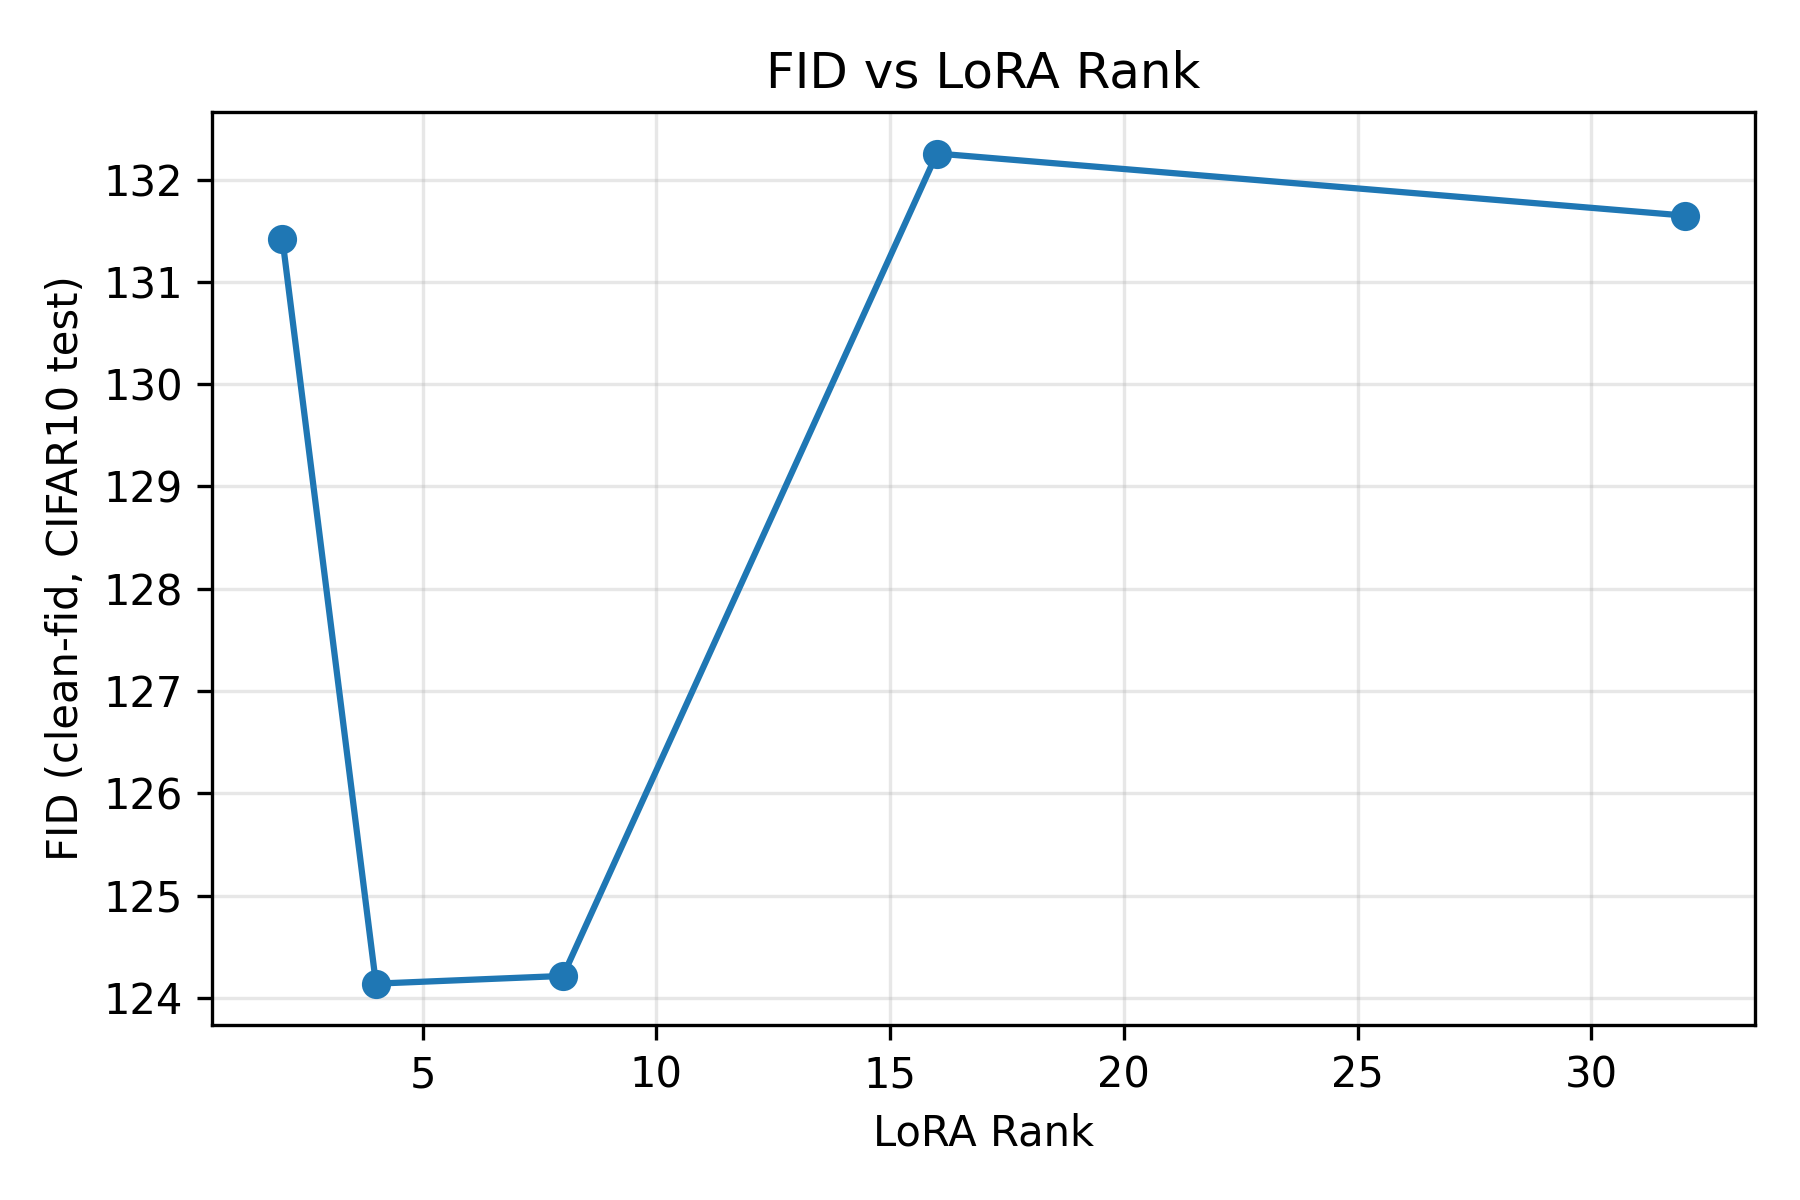
\includegraphics[width=0.85\linewidth]{../outputs/figures/fid_vs_rank.png}
  \caption{Main DDPM sweep: FID versus LoRA rank.}
  \label{fig:fid_vs_rank}
\end{figure}

\begin{figure}[t]
  \centering
  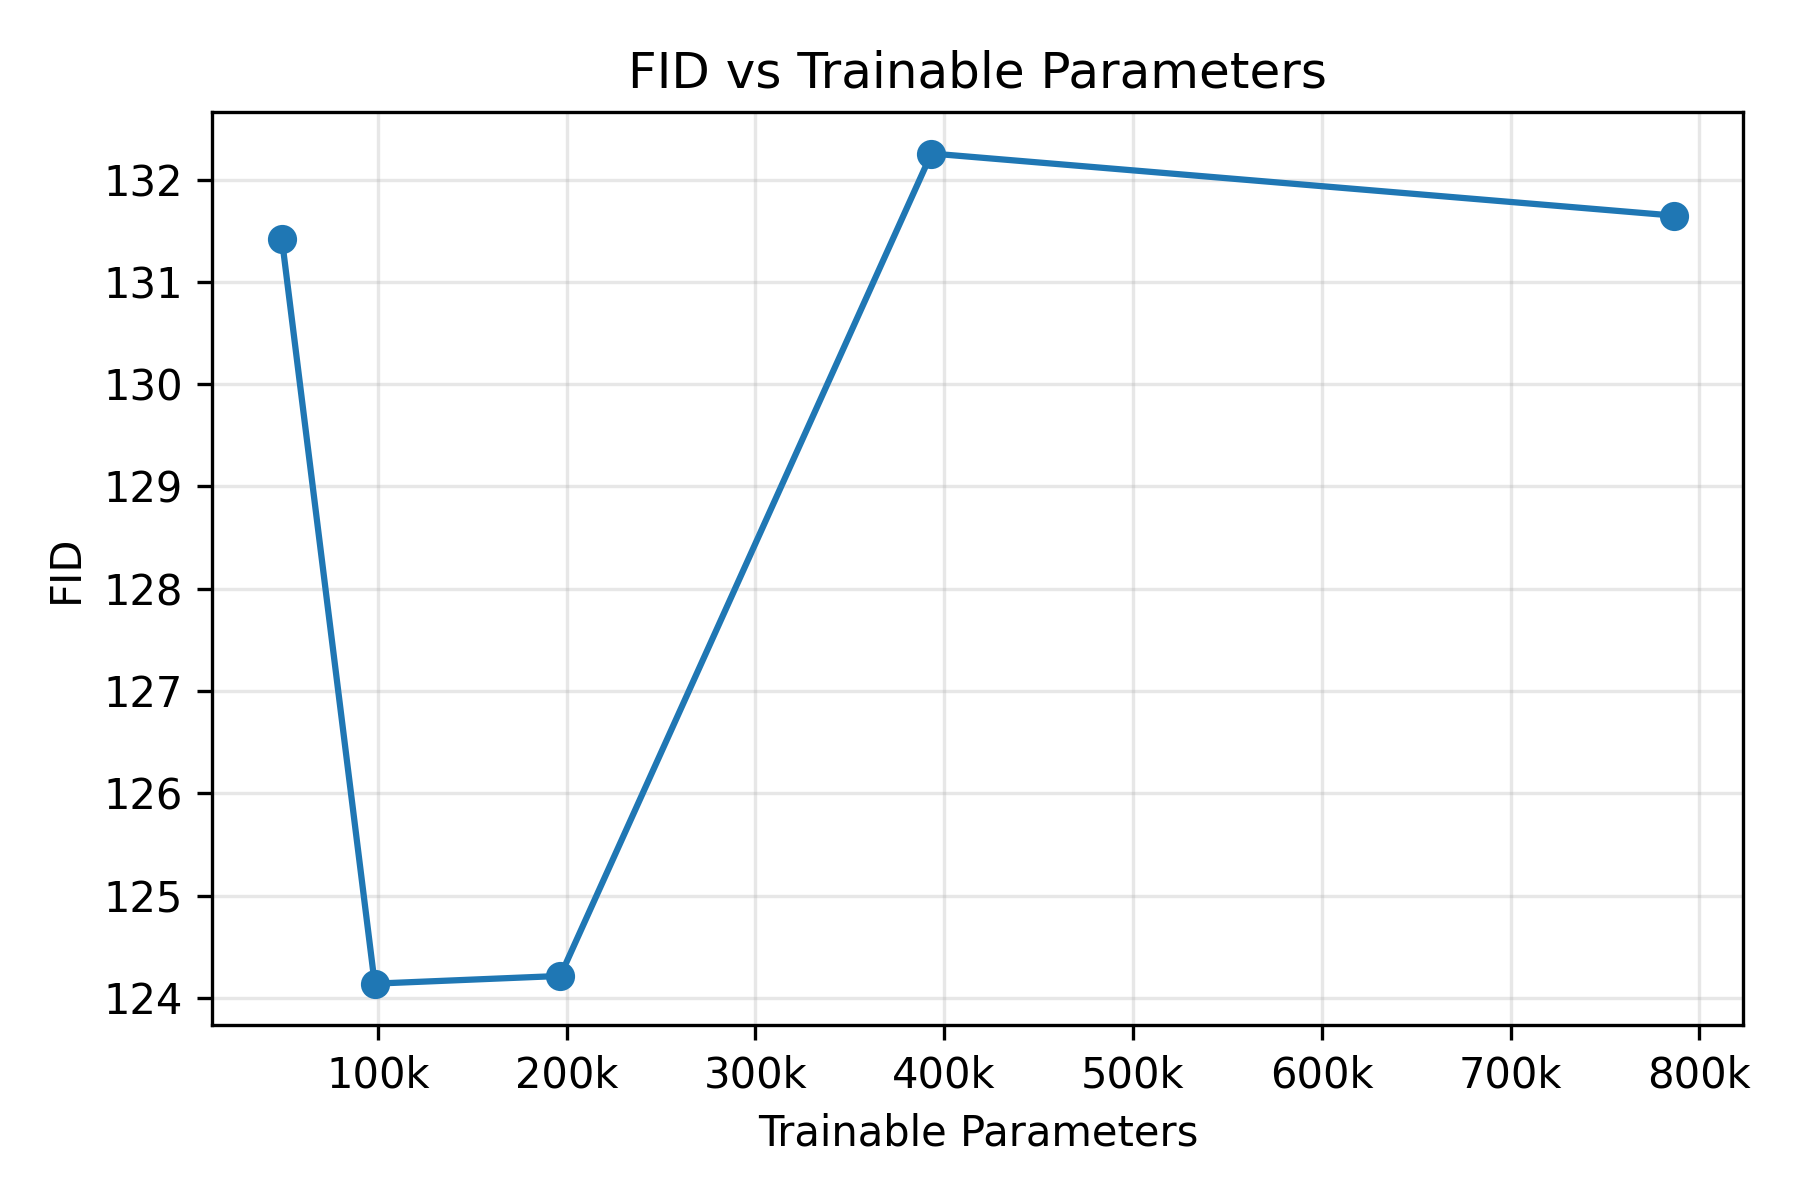
\includegraphics[width=0.85\linewidth]{../outputs/figures/fid_vs_trainable_params.png}
  \caption{Main DDPM sweep: FID versus trainable parameters.}
  \label{fig:fid_vs_trainable}
\end{figure}

The runtime and memory increases are modest but consistent with rank growth (Table~\ref{tab:main_ddpm}), while quality gains saturate quickly. This supports an engineering recommendation to prioritize moderate ranks when training budgets are fixed and tuning time is limited.
